\documentclass[12pt,a4paper]{article}
\usepackage{geometry}
\usepackage{graphicx}
\usepackage{amsmath}
\usepackage{amssymb}
\usepackage{booktabs}
\usepackage{array}
\usepackage{enumitem}
\usepackage{xcolor}
\usepackage{ulem}
\usepackage{float}
\usepackage{caption}
\usepackage[english]{babel}
\usepackage{csquotes}
\usepackage{multicol}
\usepackage[center]{titlesec}
\usepackage{fancyhdr}
\usepackage{lipsum}
\usepackage{titlesec}
\usepackage{lettrine}
% Modern font setup
\usepackage{newtxtext}
\usepackage{newtxmath}
\usepackage[T1]{fontenc}
\renewcommand{\thesection}{\Roman{section}}  % Uppercase Roman
% \renewcommand{\thesection}{\roman{section}} % Lowercase roman
\usepackage{microtype}
\usepackage{titlesec}
\microtypesetup{
    protrusion=true,
    expansion=false}
% Bibliography setup
  \renewcommand{\refname}{DAFTAR PUSTAKA}%

% Set page margins with reduced top margin
\geometry{
    left=2cm,
    right=2cm,
    top=1cm,       % Reduced from 3.5cm to 0.5cm
    bottom=3cm,
    headheight=15pt,
    headsep=0pt      % Remove additional space between header and text
}
\titleformat{\section}[block]
  {\centering\large}{\thesection}{1em}{}
\titlespacing*{\section}{0pt}{11pt}{1pt}

% Center section headings
\titleformat{\section}[block]
  {\centering\large}{\thesection}{1em}{}

% Custom commands
\newcommand{\keywords}[1]{\par\vspace{0.5\baselineskip}\noindent\textbf{Kata Kunci:} #1}
\newcommand{\smallcaps}[1]{\textsc{#1}}

% Header setup
\pagestyle{fancy}
\fancyhf{}
\renewcommand{\headrulewidth}{0pt}
\fancyhead[L]{\color{gray!70}\small Journal of Physics and Applications}
\fancyhead[R]{\color{gray!70}\thepage} % Grey page number in top right
\fancyfoot{}
\usepackage{hyperref}
\makeatletter
% Completely redefine thebibliography environment
\renewenvironment{thebibliography}[1]
     {\section*{DAFTAR PUSTAKA}%  % Force the title we want
      \@mkboth{\MakeUppercase\refname}{\MakeUppercase\refname}%
      \list{\@biblabel{\@arabic\c@enumiv}}%
           {\settowidth\labelwidth{\@biblabel{#1}}%
            \leftmargin\labelwidth
            \advance\leftmargin\labelsep
            \@openbib@code
            \usecounter{enumiv}%
            \let\p@enumiv\@empty
            \renewcommand\theenumiv{\@arabic\c@enumiv}}%
      \sloppy
      \clubpenalty4000
      \@clubpenalty \clubpenalty
      \widowpenalty4000%
      \sfcode`\.\@m}
     {\def\@noitemerr
       {\@latex@warning{Empty `thebibliography' environment}}%
      \endlist}
\makeatother
\usepackage{bookmark}
% Title and authors
\title{\fontsize{24pt}{28pt}\selectfont Gaya Selingkung dan \textit{Template} Artikel Ilmiah Jurnal Sains dan Seni ITS}
\author{
  \vspace{-3pt}\fontsize{11pt}{13pt}\selectfont Penulis P. Pertama, Penulis K. Kedua, dan Penulis K. Ketiga\\
    \vspace{-3pt}\fontsize{11pt}{13pt}\selectfont Afiliasi Penulis\\
    \fontsize{11pt}{13pt}\selectfont\textit{e-mail}: penuliskorespodensi@email.com
}
\date{}
\makeatletter
\renewcommand{\@maketitle}{%
  \newpage\null
  \vspace*{-1em}%
  \begin{center}%
    {\LARGE \@title \par}%
    \vskip 1.5em%
    {\large
      \begin{tabular}[t]{c}
        \@author
      \end{tabular}\par
    }%
    \vskip 1em%
    {\large \@date}%
  \end{center}%
  \par
  \vskip 1.5em%
}
\makeatother
\setlength{\parindent}{0em}
\begin{document}

\maketitle
\thispagestyle{fancy}

\begin{multicols}{2}
\textbf{Abstrak—Yang dimaksud gaya selingkung (in house style) adalah tatatulis yang dibakukan oleh penerbit sebuah tulisan agar tulisan-tulisan yang dimuat memiliki kesamaan gaya (style). Selanjutnya, template adalah sumber baku penulisan ilmiah yang biasanya sudah disediakan dalam bentuk file untuk memudahkan penulis memenuhi gaya selingkung yang disyaratkan. Untuk publikasi ilmiah, file ini adalah template yang berisi gaya selingkung untuk itu. Tampilan yang ada di dalam template ini, dan juga yang dituliskan penulis, tidak akan mengalami penyuntingan sebelum penerbitan. Berikut adalah gaya selingkung yang dimaksud, dimulai dari Abstrak. Abstrak dituliskan dengan paragraf tunggal. Abstrak mencakup pendahuluan, metode dan hasil yang dicapai, tanpa ada acuan pada daftar pustaka. Abstrak harus menggambarkan penelitian yang dilakukan secara ekplisit dengan kalimat yang lugas dan jelas. Abstrak dan artikel ditulis dalam bahasa Indonesia baku.  Panjang abstrak yang disarankan adalah antara 100 hingga 300 kata.}\par\vspace{0.5\baselineskip}
\textbf{Kata Kumci—keyword1,keyword2}
\section{PENDAHULUAN}
\lettrine[lines=2, lraise=-0, nindent=0pt, findent=-1pt]
{\fontsize{28pt}{28pt}\selectfont D}{}\smallcaps{OKUMEN} ini adalah \textit{template} untuk Microsoft \textit{Word} versi 6.0 ke atas. \textit{Template} ini sengaja diambilkan dan dimodifikasi dari situs \textit{IEEE} untuk \textit{Preparation of Papers for IEEE TRANSACTIONS and JOURNALS} dengan maksud agar Anda lebih dekat mengenal penulisan artikel ilmiah pada jurnal internasional.\cite{1}
\section{METODOLOGI}
\lipsum
\section{PEMBAHASAN}
\begin{table}[H]
  \centering
  \caption{Nilai \textit{constant ratio} untuk berbagai kombinasi pasangan}
  \label{tab:cr}
  \begin{tabular}{l l c}
  \toprule
  \textbf{Id} & \textbf{Pasangan} & \textbf{Rata-Rata CR*} \\
  \midrule
  \textit{R1} & a -- c1 & 0,0193233 \\
  \textit{R2} & b -- c1 & 0,0132334 \\
  \textit{R3} & c -- c1 & 0,0132334 \\
  \textit{R4} & a -- c2 & 0,2343343 \\
  \textit{R5} & b -- c2 & 0,3423423 \\
  \textit{R6} & c -- c2 & 0,3423415 \\
  \textit{R7} & a -- c3 & 0,0023444 \\
  \textit{R8} & b -- c3 & 0,0200343 \\
  \textit{R9} & c -- c3 & 0,0234443 \\
  \bottomrule
  \end{tabular}
  \end{table}
\lipsum
\begin{figure}[H]
  \centering
  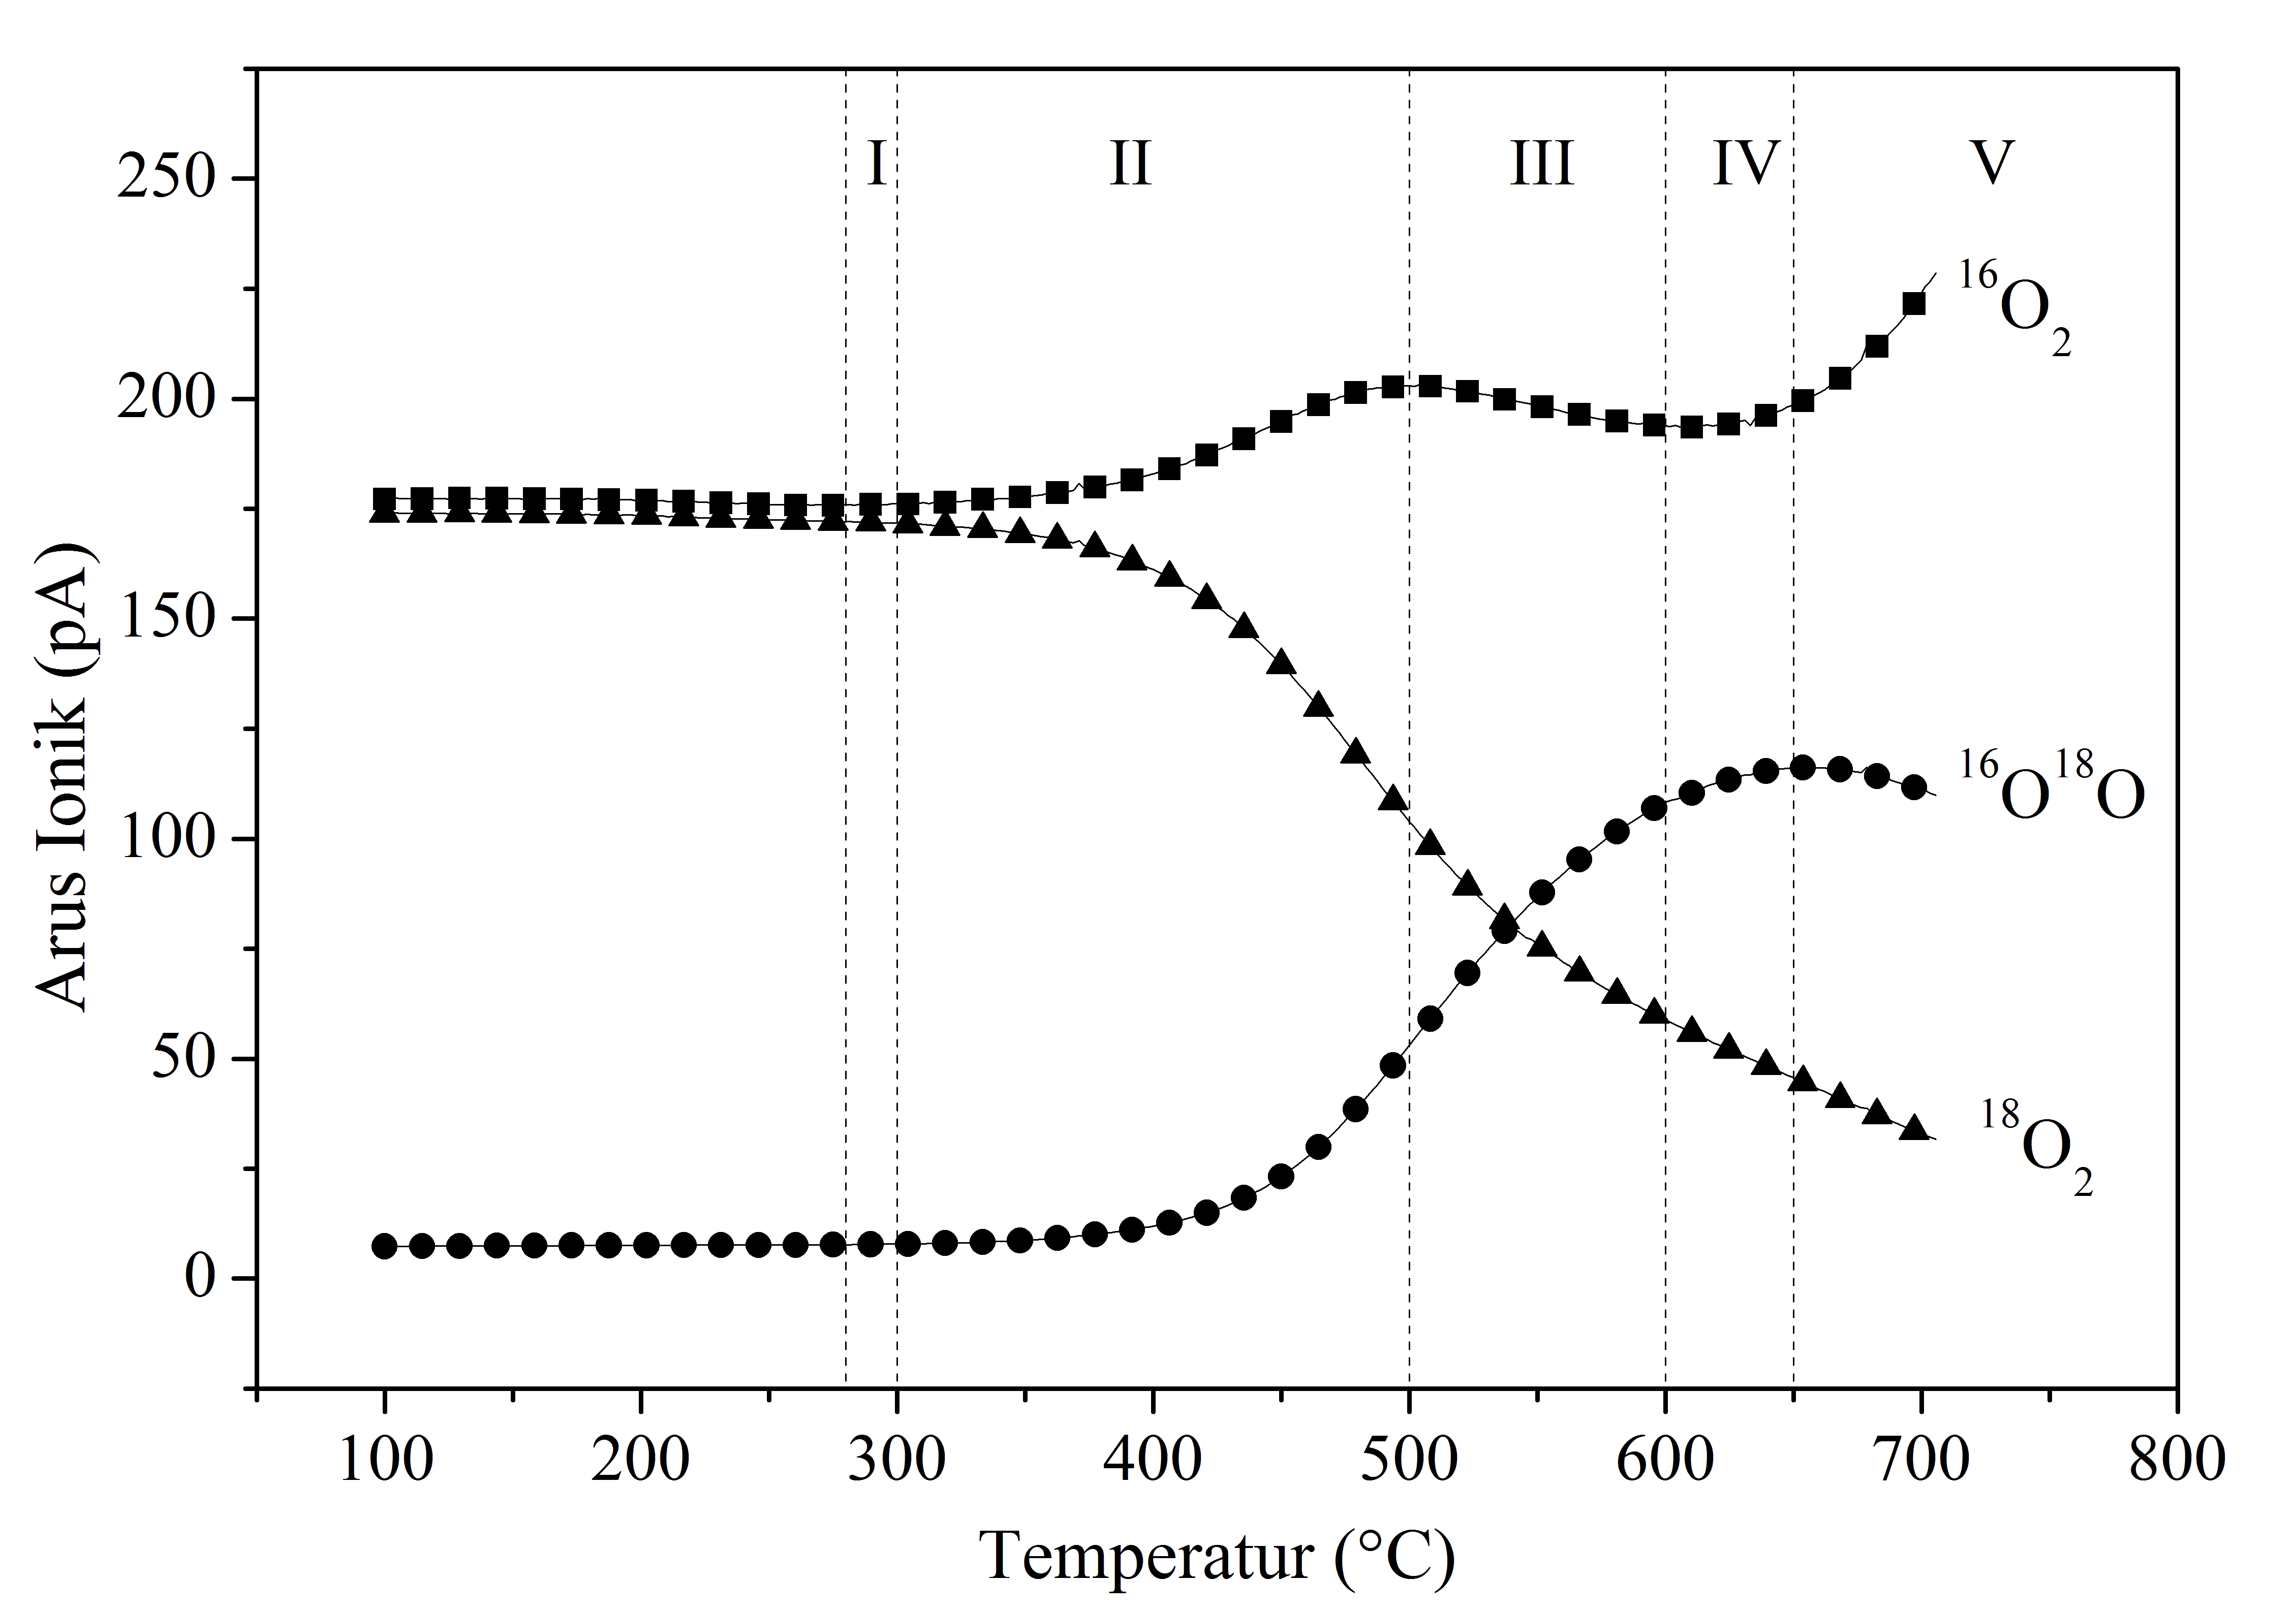
\includegraphics[width=0.7\linewidth]{fig1.png}
  \caption{Example of a inserted image}
  \label{fig:example}
\end{figure}
\section{KESIMPULAN}
\lipsum
% Bibliography
\begin{thebibliography}{99}
\bibitem{1} 
G. O. Young, ``Synthetic structure of industrial plastics,'' in \textit{Plastics}, 2\textsuperscript{nd} ed. Vol. 3, J. Peters, Ed. New York: McGraw-Hill, 1964, pp. 15--64.
\bibitem{2} 
W.-K. Chen, \textit{Linear Networks and Systems}. Belmont, CA: Wadsworth, 1993, pp. 123--135.
\end{thebibliography}

\end{multicols}
\end{document}